\documentclass{article}
\usepackage[final,sglblindworkshop]{neurips_2026}
\workshoptitle{Machine Learning for Systems}

\usepackage[utf8]{inputenc}
\usepackage[T1]{fontenc}
\usepackage[hypertexnames=false]{hyperref}
\usepackage{url}
\usepackage{booktabs}
\usepackage{graphicx}
\usepackage{float}
\usepackage{amsfonts}
\usepackage{amsmath}
\usepackage{amssymb}
\hypersetup{hidelinks}
\usepackage{placeins}


\title{ARI: Measuring Reproducibility in Deployed ML Systems}

\author{%
  The SEMQ Group \\
}

\renewcommand{\topfraction}{0.95}
\renewcommand{\bottomfraction}{0.9}
\renewcommand{\textfraction}{0.05}
\renewcommand{\floatpagefraction}{0.8}
\setcounter{topnumber}{3}
\setcounter{totalnumber}{4}
\setlength{\textfloatsep}{6pt plus 2pt minus 2pt}
\setlength{\intextsep}{6pt plus 2pt minus 2pt}
\setlength{\abovecaptionskip}{5pt}
\setlength{\belowcaptionskip}{2pt}
\renewcommand{\arraystretch}{0.90}
\AtBeginDocument{%
  \setlength\abovedisplayskip{4pt plus 1pt minus 1pt}%
  \setlength\belowdisplayskip{4pt plus 1pt minus 1pt}%
  \setlength\abovedisplayshortskip{2pt}%
  \setlength\belowdisplayshortskip{2pt}}

\begin{document}
\maketitle

\begin{abstract}
Two identical requests to the same embedding API can return numerically different vectors, yet the frequency and magnitude of this variation are generally not reported by providers. We introduce the AI Reproducibility Index (ARI), a black-box protocol that converts vector outputs into deterministic codes and measures their agreement across execution conditions. Across five commercial embedding APIs, mean exact-code agreement ranges from 0.169 to 1.000. In controlled retrieval experiments, precision and serving changes alter the codes of 47–100\% of documents while Recall@10 remains statistically indistinguishable from baseline. Under synthetic injected perturbations that preserve Recall@10 at 0.988, 11.5\% of 15-hop retrieval trajectories diverge; under bf16, less than 1\% per-token divergence changes 20.8–35.4\% of complete greedy generations. ARI exposes representation-level variation that endpoint quality metrics can otherwise miss.


\end{abstract}

\section{Introduction}\label{sec1}

Reproducibility in deployed inference depends on execution conditions. Floating-point non-associativity, kernel selection, batch shape and precision can alter outputs even without sampling [1, 2, 8, 11] (Appendix~\ref{app:batch}). Self-hosted decoding here is greedy; hosted runs request temperature zero, but their effective sampling behavior is not fully observable.

Conventional task metrics may not detect this variation: retrieval quality can remain unchanged while representations and ranked lists differ, and hosted API users lack the backend visibility to attribute a change to a mechanism. The consequence is sharpest where a system stores a discretization of an embedding rather than the embedding itself, as with semantic IDs in sequence and recommendation models [3]: the stored symbol either matches or does not, and there is no tolerance in which upstream drift can be absorbed.

ARI is a common protocol for measuring representation-level reproducibility in systems that expose vector-valued outputs: it standardizes the perturbation conditions, frozen input set, deterministic probe, and reporting rule needed to compare drift without serving-internal access. Prior work documents numerical variation in hosted embeddings [4], studies reproducibility across vector-retrieval configurations [5], and makes LLM inference deterministic by construction [6]. ARI addresses the complementary measurement problem: comparing drift across deployed systems under common, externally inducible conditions, including hosted APIs whose serving internals are unavailable.

\vspace{-4pt}\section{The ARI protocol}\label{sec2}\vspace{-2pt}

\textbf{Definitions.} The system under test is $A:\mathcal{X}\to\mathbb{R}^{d}$, mapping an input to an embedding or per-step logit vector under an explicitly fixed prefix and vocabulary. A baseline run holds the user-controlled execution axes fixed and each comparison condition varies one of them; on self-hosted systems this approximates a single-variable intervention, while on hosted APIs backend state is unobservable, so drift is reported as associated with the condition rather than attributed to a mechanism.

\textbf{The probe.} A deterministic quantizer $Q$ turns each output vector into a code with two bits per dimension, recording each coordinate's sign and whether its magnitude exceeds half a calibrated scale. $Q$ is bit-deterministic, so it contributes no disagreement of its own, and per-coordinate, so drift can be traced to specific dimensions (Appendix~\ref{app:calib}).

\textbf{Conditions.} Reproducibility is not one property, so the conditions are tiered by what the comparison holds fixed (Table~\ref{tab:conditions}, Appendix~\ref{app:conditions}). \texttt{same} is an immediate repeat (T0); \texttt{proc}, a fresh process, and \texttt{conc}, a concurrent burst against a calm pass, hold machine, kernel, hardware and model fixed (T1) and with \texttt{time}, a gap over 24\,h, form the externally observable core that any system can be asked to vary; \texttt{lib}, \texttt{mach} and \texttt{prec} (T2--T4) are self-hosted diagnostics. A T1 disagreement violates a stricter repeatability requirement than a T4 disagreement, where precision itself changed. The tiers order the conditions, not the models; on hosted APIs no tier can be held fixed, so \texttt{time} carries none.

\textbf{Metrics and their units.} For condition $c$, $\mathrm{HER}_c=n^{-1}\sum_i\mathbf 1[Q(A_0(x_i))=Q(A_c(x_i))]$. ARI-HER is the arithmetic mean over $\{\texttt{proc},\texttt{conc},\texttt{time}\}$, not the fraction matching jointly under all three; \texttt{same} is a separate control. Because exact agreement depends on vector dimension and quantizer sensitivity, HER is not always comparable across models, so ARI also reports ARI-$\hat\sigma$, a calibrated noise-equivalent scale (Appendices~\ref{app:calib} and~\ref{app:panel}). The quantizer packs several coordinates into one byte, so a mean over packed buffers is a \emph{byte} rate that overstates an isolated coordinate change by the packing factor; disagreement quantities must be read against their declared denominators (Appendix~\ref{app:units}), and HER, an equality, is unaffected.

\textbf{Scope and reporting.} The embedding API panel compares one execution pair per condition over 1{,}000 frozen inputs; auxiliary experiments use their own sample sizes, so bootstrap intervals quantify uncertainty across inputs, not across realizations of the serving environment (Appendix~\ref{app:selfhosted} replicates two conditions). We apply the protocol to embeddings (ARI-R), to per-step logits (ARI-D-internal, teacher-forced on the baseline token sequence so every condition sees identical prefixes), and to the completion bytes of hosted decoding endpoints, where no logits are exposed (ARI-D); agent outcomes are analyzed separately, without quantization. Reports carry a hash-pinned 1,000-item BEIR slice [7], an environment manifest, a result digest, and an Ed25519 signature (Appendices~\ref{app:calib}--\ref{app:verif}).

\vspace{-4pt}\section{Results}\label{sec3}\vspace{-2pt}

\vspace{-3pt}\subsection{Two black-box panels: the same providers, two layers}\label{sec:panels}\vspace{-1pt}

\begin{table}[H]
\centering\caption{Exact-code agreement across five commercial embedding APIs on the frozen inputs, $n=1{,}000$; \texttt{time} at a ${\sim}76$h gap, \texttt{conc} a 64-way burst vs calm (16-way for one rate-limited provider). ARI-HER is strict whole-code repeatability, not a dimension-normalized score (Appendix~\ref{app:panel}).}\label{tab:panel}\footnotesize\setlength{\tabcolsep}{4pt}
\begin{tabular}{lrrrrrl}
\toprule
provider / model & \texttt{same} & \texttt{proc} & \texttt{conc} & \texttt{time} & \textbf{ARI-HER} & 95\% CI \\
\midrule
gemini-embedding-001 & 1.000 & 1.000 & 1.000 & 1.000 & \textbf{1.000} & [1.000, 1.000] \\
text-embedding-3-large & 0.859 & 0.862 & 0.851 & 0.822 & \textbf{0.845} & [0.822, 0.866] \\
mistral-embed & 0.734 & 0.753 & 0.791 & \textbf{0.554} & \textbf{0.699} & [0.672, 0.727] \\
voyage-4-large & 0.571 & 0.615 & \textbf{0.209} & 0.676 & \textbf{0.500} & [0.472, 0.528] \\
embed-v4.0 & 0.133 & 0.146 & 0.130 & 0.232 & \textbf{0.169} & [0.147, 0.194] \\
\bottomrule
\end{tabular}
\end{table}

Different conditions expose different disagreement patterns: one system records 0.209 under concurrency against 0.615 in a fresh process; another falls to 0.554 only after the multi-day interval. Exact agreement penalizes wider codes, so the normalized bounds of the two lowest systems overlap and their ordering is unresolved (Appendix~\ref{app:panel}); nine self-hosted models read 1.000 on all three (Appendix~\ref{app:selfhosted}). Hosted text-generation endpoints expose no vectors, so the same conditions are applied to the completion bytes: 100 frozen prompts at temperature 0, $k=8$ repeats per prompt ($k=12$ under burst), scored as the fraction of repeat pairs that are byte-identical (Figure~\ref{fig:arid}, left; Appendix~\ref{app:arid}).

\begin{figure}[t]
\centering
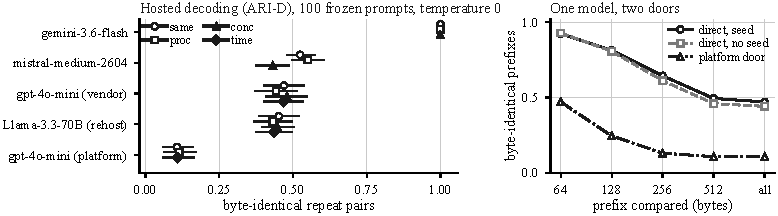
\includegraphics[width=\linewidth]{figure2.pdf}\vspace{-2pt}
\caption{Hosted decoding is a second black-box layer. \textbf{Left:} byte-identical repeat rates on five endpoints, 100 frozen prompts at temperature 0, 95\% bootstrap intervals over prompts. One vendor holds 1.0000 over 2{,}800 completions including a sustained 64-in-flight burst; the remaining measured rates are 0.107--0.550; condition intervals overlap their immediate-repeat intervals. \textbf{Right:} the same \texttt{gpt-4o-mini} snapshot on overlapping reported fingerprints through the vendor API and a platform gateway: half as byte-stable at 64 bytes, four times less over full completions, with a separate no-seed control on the vendor API.}
\label{fig:arid}
\end{figure}

For the three providers measured on both layers, agreement is ordered the same way; this descriptive concordance does not identify a shared mechanism. On hosted decoding, condition intervals overlap immediate-repeat intervals, which does not establish equivalence. A gateway reporting the same model snapshot as the vendor API is less byte-stable even at fixed prefix lengths; a no-seed vendor control does not close the gap. The gateway ignores the tested sampling-parameter block, so effective sampling remains confounded. Shared fingerprints do not establish identical backend execution (Appendix~\ref{app:arid}).

\vspace{-5pt}\subsection{Recall@10 may not detect large representation drift}\label{sec:blind}\vspace{-1pt}

BEIR SciFact (5{,}183 documents, 300 judged queries), all-MiniLM-L6-v2; reference fp32/CPU/4-thread/batch-32, every other condition changing one thing in a fresh process; paired bootstrap over queries, 10{,}000 resamples (Appendix~\ref{app:scifact}).

\begin{figure}[t]
\centering
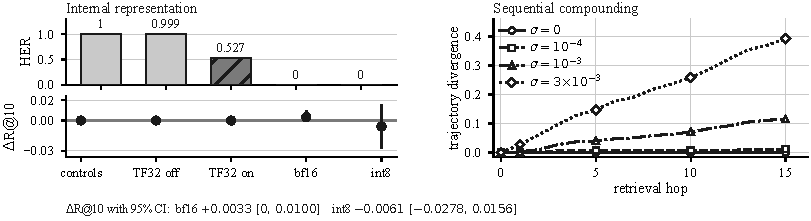
\includegraphics[width=\linewidth]{figure1.pdf}\vspace{-3pt}
\caption{The measurement gap and its downstream cost. \textbf{Left:} on BEIR SciFact, process, thread and batch changes leave every code intact, while precision and compute-mode changes alter the codes of 47--100\% of documents, yet no $\Delta$Recall@10 interval excludes zero (values printed below the panel). \textbf{Right:} per-hop noise small enough to pass the predefined clean-ranking overlap threshold ($\sigma=10^{-3}$, clean top-10 overlap $=0.988$) diverts 11.5\% of 15-hop trajectories; at $\sigma=0$ divergence is 0 at every depth.}
\label{fig:overview}
\end{figure}

Under bf16, fp16 and int8, HER falls to 0 while every Recall@10 interval includes zero; a fresh process, a single thread, and batch sizes of 8 and 128 each leave every code intact (HER $=1.000$) on this host. Relative to the CPU fp32 reference, GPU fp32 with TF32 enabled changes 47\% of document codes while \(\Delta R@10=0\). Turning TF32 off restores 0.9992, and a 2x2 over TF32 $\times$ \texttt{use\_deterministic\_algorithms} isolates it (HER 1.000 off, 0.749 on; the flag has no effect), consistent with TF32's reduced mantissa amplifying otherwise smaller differences past the probe threshold.

\textbf{Batch controls depend on the host.} On H100, four of seven encoders disagree at batch 1 against a batch-32 reference with TF32 off: three have HER 0.9990 and mxbai-embed-large-v1 has 0.5560. All 21 same-batch control cells have HER 1.0000, supporting batch-associated variation. Deterministic algorithms do not remove it; kernel attribution needs profiling (Figure~\ref{fig:batch}, Appendix~\ref{app:batch}).

\vspace{-6pt}\subsection{Small per-step divergence compounds into outcome divergence}\label{sec:compound}\vspace{-1pt}

\textbf{Iterative retrieval (controlled stress test).} A self-avoiding nearest-neighbor walk uses cached bge-large-en-v1.5 embeddings of NFCorpus documents as successive queries. Independent synthetic Gaussian query noise at $\sigma=10^{-3}$ changes 11.5\% of 3{,}000 trajectories by hop 15, while clean top-10 overlap on a separate sample is 0.9879 (Figure~\ref{fig:overview}, right). This overlap is not relevance-based Recall@10. Cumulative divergence is monotone by definition; the noiseless control is zero. Structured GPU residuals [8] may behave differently, so this demonstrates possible accumulation rather than predicted API behavior (Appendix~\ref{app:walk}).

\textbf{Decoding.} On the full-vocabulary logit vector at each greedy step (48 prompts, ${\sim}2{,}265$ scored steps per model, fp32 reference, same GPU; Table~\ref{tab:decoding}), under TF32 every logit code changes while all free generations remain identical; one teacher-forced argmax differs on Qwen. Batching a prompt with three others --- as can occur during serving --- leaves the emitted tokens untouched on all three models and still moves 19--67\% of the logit codes, the batch-shape mechanism of \S\ref{sec:blind} one layer up. Under bf16 fewer than 1\% of tokens change but 20.8--35.4\% of complete generations differ, a 26--45x ratio between different units of measurement. A changed token can alter subsequent prefixes, but these rates alone do not identify causal amplification. Appendix~\ref{app:deccontrol} gives controls and the saturation caveat at this vocabulary width; Appendix~\ref{app:adversarial} compares the probe with cheaper statistics.

\begin{table}[t]
\centering\caption{ARI-D-internal, range over Llama-3.1-8B, Qwen2.5-7B and Mistral-7B-v0.3 (one L40S); ``early warning'': unchanged token, changed code. Per model: Appendix~\ref{app:deccontrol}.}\label{tab:decoding}\scriptsize\setlength{\tabcolsep}{3pt}
\begin{tabular}{lrrrr}
\toprule
condition & token agreement & HER & early warning & generations identical \\
\midrule
\texttt{proc} / 1 thread / TF32 off & 100.00\% & 1.0000 & 0.00\% & 48/48 (all three) \\
\textbf{TF32 on} & 99.96--100.00\% & 0.0000 & 99.96--100.00\% & 48/48 (all three) \\
\textbf{batched (padded batch of 4)} & 100.00\% & \textbf{0.3347--0.8065} & \textbf{19.35--66.53\%} & 48/48 (all three) \\
fp16 & 99.74--99.91\% & 0.0000 & 99.74--99.91\% & 43--47 of 48 \\
\textbf{bf16} & 99.21--99.52\% & 0.0000 & 99.21--99.52\% & \textbf{31--38 of 48} \\
\bottomrule
\end{tabular}
\end{table}

\textbf{Limitations.} API estimates rest on a single realization of each condition (Appendix~\ref{app:selfhosted} replicates two) and are not long-run drift rates. Neither decoding experiment separates drift from sampling above temperature 0, and two hosted subjects lack their \texttt{time} cell. ARI measures representation change, not harm. Appendix~\ref{app:limits} lists further limitations; Appendices~\ref{app:bounds} and~\ref{app:adversarial} report claims narrowed by our own adversarial testing.

\vspace{-5pt}\section{Conclusion}\label{sec5}\vspace{-2pt}

ARI specifies a frozen input set, deterministic probe, execution conditions and reporting rules for representation-level reproducibility. Five commercial embedding APIs span ARI-HER 0.169--1.000 in the measured captures. On SciFact, precision and compute-mode changes alter 47--100\% of document codes without a detected Recall@10 difference; GPU batch changes also alter embedding and logit codes. Representation changes need not imply harm, and whole-code equality depends on dimension and probe resolution. Hosted byte-level repetition provides a complementary observation where vectors are unavailable. These measurements support ARI as a complement to task evaluation, while repeated environment captures and validated calibration are needed for long-run rates and cross-model magnitude comparisons.\label{bodyend}


\section*{References}
\small

[1] He, H. and Thinking Machines Lab.
Defeating Nondeterminism in LLM Inference.
\emph{Thinking Machines Lab: Connectionism}, September 2025.
\url{https://doi.org/10.64434/tml.20250910}.

[2] Yuan, J., Li, H., Ding, X., Xie, W., Li, Y.-J., Zhao, W.,
Wan, K., Shi, J., Hu, X., and Liu, Z.
Understanding and Mitigating Numerical Sources of Nondeterminism
in LLM Inference.
\emph{arXiv preprint arXiv:2506.09501}, 2025.
\url{https://arxiv.org/abs/2506.09501}.

[3] Rajput, S., Mehta, N., Singh, A., Keshavan, R. H., Vu, T.,
Heldt, L., Hong, L., Tay, Y., Tran, V. Q., Samost, J., Kula, M.,
Chi, E. H., and Sathiamoorthy, M.
Recommender Systems with Generative Retrieval.
In \emph{Advances in Neural Information Processing Systems 36
(NeurIPS)}, 2023.
\url{https://proceedings.neurips.cc/paper_files/paper/2023/hash/20dcab0f14046a5c6b02b61da9f13229-Abstract-Conference.html}.

[4] OpenAI.
Embeddings with OpenAI ``text-embedding-ada-002'' Are Not Deterministic.
\texttt{openai/openai-python}, issue \#868, 2023.
\url{https://github.com/openai/openai-python/issues/868}.

[5] Wang, B., Zhao, D., Tallent, N. R., and Guo, L.
On the Reproducibility Limitations of RAG Systems.
\emph{arXiv preprint arXiv:2509.18869}, 2025.
\url{https://arxiv.org/abs/2509.18869}.

[6] Gond, R., Kamath, A. K., Ramjee, R., and Panwar, A.
LLM-42: Enabling Determinism in LLM Inference with Verified Speculation.
\emph{arXiv preprint arXiv:2601.17768}, 2026.
\url{https://arxiv.org/abs/2601.17768}.

[7] Thakur, N., Reimers, N., R{\"u}ckl{\'e}, A., Srivastava, A., and Gurevych, I.
BEIR: A Heterogeneous Benchmark for Zero-shot Evaluation of Information Retrieval Models.
In \emph{Proceedings of the Neural Information Processing Systems Track on Datasets and Benchmarks}, 2021.
\url{https://arxiv.org/abs/2104.08663}.

[8] Yashwanth, T. S.
On the Structure of Floating-Point Noise in Batch-Invariant GPU
Matrix Multiplication.
\emph{arXiv preprint arXiv:2511.00025}, 2025.
\url{https://arxiv.org/abs/2511.00025}.

[9] Ahmad, W. U., Ludwig, N., Majumdar, S., and Ginsburg, B.
Open-SWE-Traces: Advancing Dual-Mode Multilingual Distillation for Software Engineering Agents.
\emph{arXiv preprint arXiv:2606.16038}, 2026.
\url{https://arxiv.org/abs/2606.16038}.

[10] The SEMQ Group.
ARI: An Auditable Retrieval Instability Harness.
Software repository, 2026.
\url{https://github.com/The-SEMQ-Group/semq-ari-benchmark}.
Tag \texttt{v0.1-preview}.

[11] Riach, D.
Determinism in Deep Learning.
GPU Technology Conference (GTC) Silicon Valley, talk S9911, 2019.
\url{https://developer.nvidia.com/gtc/2019/video/s9911}.
See also NVIDIA, \texttt{framework-reproducibility},
\url{https://github.com/NVIDIA/framework-reproducibility}.

[12] Somepalli, G., Fowl, L., Bansal, A., Yeh-Chiang, P., Dar, Y.,
Baraniuk, R., Goldblum, M., and Goldstein, T.
Can Neural Nets Learn the Same Model Twice? Investigating Reproducibility
and Double Descent from the Decision Boundary Perspective.
\emph{arXiv preprint arXiv:2203.08124}, 2022.
\url{https://arxiv.org/abs/2203.08124}.

[13] Hochlehnert, A., Bhatnagar, H., Udandarao, V., Albanie, S.,
Prabhu, A., and Bethge, M.
A Sober Look at Progress in Language Model Reasoning: Pitfalls and Paths
to Reproducibility.
\emph{arXiv preprint arXiv:2504.07086}, 2025.
\url{https://arxiv.org/abs/2504.07086}.

[14] Iakymchuk, R., Defour, D., Collange, S., and Graillat, S.
Reproducible and Accurate Matrix Multiplication.
In \emph{SCAN: Scientific Computing, Computer Arithmetic and Validated
Numerics}, W\"urzburg, Germany, pages 126--137, 2014.
\url{https://hal.science/hal-01539180v1}.

\normalsize
\appendix

\section{Condition set}\label{app:conditions}

\begin{table}[H]
\centering\caption{ARI execution conditions, grouped by reproducibility tier. \texttt{proc}, \texttt{conc} and \texttt{time} form the externally observable core; the others are controls and self-hosted diagnostics.}\label{tab:conditions}\footnotesize\setlength{\tabcolsep}{4pt}
\begin{tabular}{cllp{0.42\linewidth}}
\toprule
tier & id & varied condition & variation potentially exposed \\
\midrule
T0 & \texttt{same} & immediate repeat & within-session repeatability \\
T1 & \texttt{proc} & fresh process & process-dependent execution (self-hosted); client state (API) \\
T1 & \texttt{conc} & concurrent burst & load-associated batching, composition, routing, queueing \\
T2 & \texttt{lib} & library version & kernel selection and library drift (self-hosted diagnostic) \\
T3 & \texttt{mach} & host & hardware change (self-hosted diagnostic) \\
T4 & \texttt{prec} & precision or compute mode & TF32, bf16, fp16, int8 (self-hosted diagnostic) \\
--- & \texttt{time} & wall-clock gap $>24$\,h & time-associated drift; backend cause unobserved \\
\bottomrule
\end{tabular}
\end{table}

\section{Probe and calibration specifics}\label{app:calib}

\textbf{The quantizer.} $Q$ is a four-level symmetric scalar quantizer (SEMQ QUANT) with one model-specific scale $s$, calibrated once as the 99th percentile of absolute coordinate values pooled over a published reference batch. Each coordinate becomes two semantically defined indicators, $Q_s(x_j)=\bigl(\mathbf 1[x_j\ge0],\,\mathbf 1[|x_j|\ge s/2]\bigr)$ --- sign and magnitude region --- for exactly two bits per dimension; the interior edge falls at $s/2$ because two equal-width magnitude bins partition $[0,s]$. With $P=Q\circ A$, all reported quantities are computed on the codes $P(x)$. The decoding-layer experiments use the same operator at eight magnitude bins, four bits per coordinate; the two probes are specified, calibrated and reported separately and their storage and detection results are never pooled.

\textbf{Response model.} Let $\rho$ be the coordinate change fraction: the fraction of coordinates whose two-bit code differs. Within the calibrated regime,
\[
\mathbb E[\rho]=\kappa\sqrt{2d/\pi}\,\sigma^{b},
\qquad
\hat{\sigma}=\left(\frac{\rho}{\kappa\sqrt{2d/\pi}}\right)^{\!1/b},
\]
with $b$ and $\kappa$ fitted per model; across 13 architectures the exponents have mean $0.979$ and standard deviation $0.028$, and $\kappa\in[0.37,0.76]$. ARI-$\hat\sigma$ averages $\rho$ over the core conditions and inverts once, equivalently pooling all comparisons; inverting per condition and averaging differs by under $1\%$ and preserves the ordering. $\hat\sigma$ is a per-coordinate scale: it normalizes the probe-response model's dependence on dimension and sensitivity, not the vector-level perturbation, which at fixed $\sigma$ grows as $\sqrt d$. It is not a direct estimate of arbitrary serving noise.

\textbf{Calibration model.} Noise is added to the raw representation before any re-normalization: re-normalizing would fold $\sigma$ back onto the unit sphere and mask the linear regime. $\sigma$ is dimensionless, a per-coordinate standard deviation expressed as a fraction of the mean representation norm over the reference batch; the corresponding vector-level perturbation grows as $\sigma\sqrt d$, so $\hat\sigma$ should be read as a per-coordinate scale rather than a relative $L_2$ magnitude.

\textbf{From bits to coordinates.} Reports currently store $\bar H$, the mean changed-bit count, from which the coordinate change fraction follows only up to the exact bound $\bar H/2d\le\rho\le\bar H/d$: a changed coordinate flips one of its two indicators or both. Rather than assume the low-drift limit $\rho\approx\bar H/d$, we propagate both endpoints, so the normalized table reports conversion bounds, rather than statistical confidence intervals. Calibration-fit uncertainty and byte-rate approximations are additional sources of error. Serializing $\rho=\tfrac1d\sum_j\mathbf 1[Q(x_j)\neq Q(x_j')]$ directly, and refitting $(b,\kappa)$ against it, removes the interval entirely; that is a v0.2 change to the report schema and the published fingerprints. The reference implementation compares packed bytes (four coordinates each) and the signer registry stores fingerprints in that convention, $4\kappa$; a factor-of-four conversion approximately preserves $\hat\sigma$ only when changed coordinates rarely share a byte. Historical byte-rate fits need validation against coordinate counts; the intervals below do not include that approximation or calibration-fit uncertainty.

\textbf{Sensitivity spread.} Measured influence spread is 1.00 for quantile binning versus about 16 for a block-microscaled format like NVFP4, whose shared per-block scale smears one perturbed dimension across its whole block. A diagonal sensitivity Jacobian is what lets drift attribute back to specific dimensions.

\section{Measurement units: bytes, bits, coordinates}\label{app:units}

The reference implementation compares packed code buffers, and the quantizer packs whether or not the calling context asks it to: at two bits per coordinate four coordinates share a byte, at four bits two do. A mean taken over two such buffers, $(\text{cur}\neq\text{ref}).\text{mean}()$, is therefore a byte disagreement rate. Four published measurements reported that quantity as a symbol or coordinate rate. Changing exactly one coordinate of 4{,}096 gives a byte rate of $4.88\times10^{-4}$ against a true coordinate rate of $2.44\times10^{-4}$: a 2x overstatement at four bits per coordinate and 4x at two. The factor falls toward one as changes become dense, so a published number cannot be converted after the fact.

The implementation now reports each quantity against its own denominator --- whole-code equality, changed coordinates (count, fraction and indices), bit Hamming over code bits only, and the byte rate under a name that says bytes --- and compares a vocabulary encoded in chunks without reading one chunk's padding as the next chunk's coordinates. HER and the aggregate ARI are exact-code equalities and are unchanged by this correction, as is $\bar H$ in the panel reports, which was already a bit count. The affected quantities are the decoding-matrix and rank-profile disagreement rates, which now appear under both names, and stored result files keep the names they were written with. The report schema gained optional \texttt{bits\_per\_coordinate}, \texttt{n\_coordinates}, \texttt{n\_bits} and \texttt{bit\_hamming\_rate} fields; no existing field changed meaning, so reports signed before the change still validate and were not re-signed.

\section{Verifiability details}\label{app:verif}

The frozen input set is a 1{,}000-item BEIR slice spanning medical, scientific and financial domains, pinned by content hash. Each report carries per-condition HER, $\bar H$ and bootstrap CI, an environment manifest, and a SHA-256 audit digest over the code matrix in fixed input order. The Ed25519 signature covers a canonical JSON serialization (fixed key order and separators) of a manifest that carries the report's SHA-256 alongside the input digest, so the signature attests to the result and the input set jointly; signing only the input digest would attest to neither HER nor $\bar H$. The signing key is held in AWS KMS and listed in a public signer registry, and the standalone verifier uses the Python standard library and \texttt{cryptography}, without importing the ARI measurement package or SEMQ. It verifies signature and artifact integrity, not the correctness of reported measurements; signer identity requires a trusted registry.

\section{The hosted decoding panel}\label{app:arid}

\textbf{Design.} 100 frozen prompts across five buckets (factual QA, code generation, instruction following, multi-step reasoning, open-ended prose), temperature 0 with a seed where the endpoint accepts one, $k=8$ repeats per prompt per condition and $k=12$ under burst. The unit is a repeat \emph{pair}: \texttt{exact\_generation} is the fraction of the $\binom{k}{2}$ pairs per prompt whose completions are byte-identical, averaged over prompts, with a bootstrap interval over prompts. \texttt{time} pairs two batches $k\times k$ across a $>24$h gap. Every figure is recomputable from a digest-bound transcript retained in the manifest.

\begin{table}[h]
\centering\caption{Byte-identical repeat rates on five hosted text-generation endpoints, 100 frozen prompts, temperature 0. ARI-D is the mean over the core $\{\texttt{proc},\texttt{conc},\texttt{time}\}$ and is withheld where a core cell is not yet measured.}\label{tab:arid}\footnotesize\setlength{\tabcolsep}{4pt}
\begin{tabular}{llrrrrr}
\toprule
endpoint & class & \texttt{same} & \texttt{proc} & \texttt{conc} & \texttt{time} & \textbf{ARI-D} \\
\midrule
gemini-3.6-flash & vendor & 1.000 & 1.000 & 1.000$^{64}$ & --- & --- \\
mistral-medium-2604 & vendor & 0.525 & 0.550 & 0.432$^{16}$ & --- & --- \\
gpt-4o-mini & vendor & 0.470 & 0.443 & 0.479$^{64}$ & 0.469 & \textbf{0.464} \\
Llama-3.3-70B-Turbo & rehosted & 0.452 & 0.431 & 0.448$^{64}$ & 0.435 & \textbf{0.438} \\
gpt-4o-mini & platform & 0.107 & 0.115 & --- & 0.109 & --- \\
\bottomrule
\end{tabular}
\end{table}

Superscripts give the achieved in-flight burst. Mistral's tier caps at 50 requests per minute, so its \texttt{conc} ran at 16; the platform org is rate-capped and has no \texttt{conc} cell at all. Intervals are in Figure~\ref{fig:arid}. No condition on any subject separates from that subject's own \texttt{same} under the CI-overlap rule.

\textbf{Calibration verdicts fixed by this run.} (i) \emph{Burst size.} $\{16,64,128\}$ on the rehosted endpoint, $k=12$ per arm, achieved in-flight peak equal to the request in every arm and zero reconnects; no arm separates from \texttt{same}, so the panel-wide burst freezes at 64, continuous with the representation layer. (ii) \emph{Length confounder.} Spearman $\rho$ between pair byte length and normalized first divergence is weak in every bucket, $|\rho|\le0.18$ with inconsistent sign, so length does not dominate the signal. (iii) \emph{Set discrimination.} The \texttt{same} floor spans 0.041 (open-ended prose) to 0.759 (instruction following), the inverse of the top-2 margin distribution across the same buckets (median 2.0 against 11.5 nats): flips concentrate where margins are thin, and no bucket saturates. \texttt{topk\_logprob\_overlap} reads 0.961 where logprobs are exposed --- the distributions agree almost entirely until the flip.

\textbf{The platform door.} The gateway resolves, per the response's own passthrough metadata, to \texttt{gpt-4o-mini-2024-07-18}, and 6 of its 12 \texttt{system\_fingerprint} values also appear in the direct run's 45. Its \texttt{parameters} block is accepted and discarded: \texttt{temperature} and \texttt{maxTokens} have no effect, non-numeric values in either field return 200, and \texttt{maxTokens: 8} against a long-essay prompt returned 250 completion tokens with \texttt{finish\_reason: stop}. Because \texttt{maxTokens} is ignored its completions run longer (mean 1{,}050 against 440 bytes) and mechanically have more room to diverge, so Figure~\ref{fig:arid} (right) compares byte-identical \emph{prefixes} at fixed horizons instead; the gap survives at every horizon. The seed is the other candidate confounder --- the direct run sends one and the platform cannot accept one --- and a dedicated no-seed arm on the direct door reads 0.441 against 0.470, within noise at every prefix horizon. All 12 of the platform's day-one fingerprints reappear on day two, so its \texttt{time} cell remains near its immediate-repeat rate; stable fingerprints cannot exclude unreported backend changes. The residual is not attributable from outside: the door's effective sampling parameters, prompt handling and trust-layer processing are all invisible to the caller, and that non-attributability is the finding for this class rather than a gap in the analysis.

\textbf{Power.} A 252-cell simulation (200 trials per cell, 500 bootstrap resamples per arm) sizes what the CI-overlap rule can detect at 100 prompts. At a noisy baseline (floor 0.7--0.9) a $0.10$ drop in exact-generation is detected with power 0.89--0.96 when deviations are bimodal, but only 0.53--0.55 when they are unique and concentrated on a subset of prompts; a $0.05$ drop is detected at 0.04--0.26. False-positive rates are at most 1\% across the grid. Raising repeats from 8 to 12 does not fix the concentrated case; more prompts is the relevant design change. A verdict of ``$\approx$ same'' therefore does not exclude a concentrated $0.10$ decrease, and the rule trades power for a low false-positive rate deliberately.

\section{Batch invariance and non-associativity}\label{app:batch}

\textbf{Non-associativity, measured directly.} Over 50{,}000 random triples drawn at coordinate scale 0.1, $(a+b)+c\neq a+(b+c)$ for 16{,}015 triples in fp32 (32.0\%, max absolute difference $5.96\times10^{-8}$) and 15{,}922 in fp16 (max $4.88\times10^{-4}$). Summing one fixed 1{,}024-term vector in 32 random orders gives 31 distinct fp32 results with a spread of $5.85\times10^{-7}$, against a float64 reference error of $3.98\times10^{-7}$; at width 384 it gives 8 distinct results. This is the mechanism of \S\ref{sec1}, not a model-level finding, and it is included as an illustration of one numerical mechanism, rather than an attribution of every measured condition.

\textbf{The sweep.} Seven encoders on \texttt{p5.48xlarge} (8x H100, Hopper), torch 2.5.1+cu121, 1{,}000 frozen inputs, fixed QBIN scale from the published registry, one process per capture, batch 32 as the reference inside each cell. \texttt{BAAI/bge-m3} is excluded: it ships no safetensors and transformers 5.x refuses to \texttt{torch.load} a \texttt{.bin} under torch $<$ 2.6, and upgrading torch for one model would change the kernels for every other model in the table, which is what the table measures.

\begin{figure}[h]
\centering
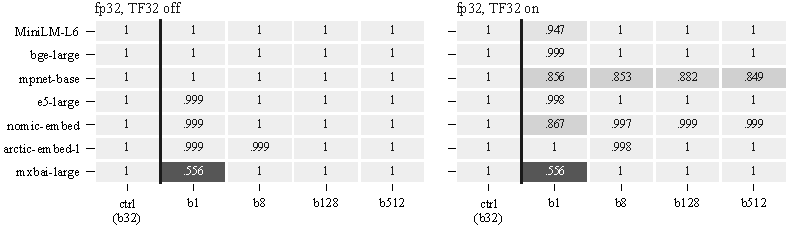
\includegraphics[width=\linewidth]{figure3.pdf}\vspace{-2pt}
\caption{HER against a batch-32 reference on H100, at fp32. The \texttt{ctrl} column captures batch 32 twice in separate processes and compares them: all 21 cells read exactly 1.0000, supporting batch-associated differences; finite repeat controls do not exclude all capture variation. Batch sensitivity is real and concentrated at batch 1, where changed computation shapes can select different kernels; no kernel trace is reported here. The deterministic-algorithms cell (not shown) is bit-identical to the left panel for all seven models at every batch size. all-mpnet-base-v2 under TF32 is the exception: it disagrees at every batch size with no ordering by batch.}
\label{fig:batch}
\end{figure}

A two-encoder boundary sweep under TF32 places the effect precisely: all-MiniLM-L6-v2 reads 0.9470 at batch 1, 0.9990 at batch 2 and 1.0000 from batch 4 upward. The whole table reproduced value for value on a second instance of the same type. Two results are not explained here. mxbai-embed-large-v1 reads exactly 0.5560 at batch 1 in all three cells, with TF32 on and off, which makes it precision-independent; it is also the outlier of the cross-GPU comparison in Appendix~\ref{app:selfhosted}, at 0.5371 against CPU. And TF32's effect on batch sensitivity does not resolve cleanly: it lowers agreement on two models, leaves one unchanged and raises one. Cells are never compared across rows, since they differ in more than batch size.

\section{Iterative retrieval stress-test details}\label{app:walk}

A self-avoiding nearest-neighbor walk over NFCorpus (3{,}633 documents), using bge-large-en-v1.5, selects the nearest unvisited document and uses its cached embedding as the next query. The corpus embeddings are fixed; synthetic isotropic Gaussian noise is added independently to the query at each hop. Over 100 seed documents and 30 runs per seed, 11.5\% of trajectories differ from the noiseless reference by hop 15 at $\sigma=10^{-3}$ (Figure~\ref{fig:overview}, right). This is the largest tested noise level meeting a predefined clean top-10 overlap threshold of 0.98; the measured overlap is 0.9879 on a separate 200-document sample with 30 noise draws each. This overlap is not relevance-based Recall@10 as used on SciFact. Divergence counts the fraction of 3{,}000 seed/run prefixes that differ by each depth and is necessarily nondecreasing; monotonicity alone is not evidence of amplification. The noiseless control has zero divergence. GPU residuals can be structured rather than isotropic [8], so this illustrates possible accumulation in a retrieval walk, not predicted API or agent behavior. The experiment is \texttt{L3\_09\_agentic\_compounding} in the companion \texttt{semq-research} repository; its archived run is identified in the review notes.

The archived analysis, configuration, environment, replay instructions and checksum manifest are retained in \texttt{docs/paper/evidence/L3\_09\_agentic\_compounding}. Figure~\ref{fig:overview} verifies the manifest hashes before reading the aggregate curves. The bundle does not retain individual trajectories, so seed-level uncertainty cannot be reconstructed. Its configuration requests a 3{,}000-document limit while its analysis reports 3{,}633 documents; exact replay requires resolving the historical handling of this setting. Replay identifies a container digest but no source Git revision.

\section{Outcome-layer reproducibility (ARI-E)}\label{app:arie}

ARI-E applies the same discipline --- repeat, control, attribute --- to agent outcomes on \texttt{nvidia/Open-SWE-Traces} [9]: two scaffolds (SWE-agent, OpenHands) crossed with two models over ${\sim}18{,}000$ SWE-bench-style instances, up to three rollouts each, graded by each repository's own test suite. An outcome is the recorded test verdict. Agreement on this binary outcome does not establish identical patches, trajectories or task correctness beyond the tests; judge-based grading would introduce a different source of measurement variability.

The estimator is an agreement gap, not a corrected success rate. On instances with at least two rollouts per side, let $D_{\text{cross}}$ be the rate at which paired verdicts differ across the two conditions and $D_{\text{self}}$ the rate at which repeated rollouts differ within one; we report $\Delta=D_{\text{cross}}-D_{\text{self}}$.

\begin{table}[h]
\centering\caption{Self-consistency and cross-condition agreement across four scaffold and model contrasts. The last column is the share of the raw cross-condition disagreement that the self-consistency control removes.}\label{tab:arie}\scriptsize\setlength{\tabcolsep}{3.5pt}
\begin{tabular}{lrrrrlr}
\toprule
contrast & cases & self-consistency & cross agreement & $\Delta$ & 95\% CI & removed \\
\midrule
scaffold, model = Qwen3.5-122B & 10{,}788 & 0.874 & 0.785 & \textbf{+0.089} & [+0.083, +0.094] & 59\% \\
scaffold, model = Minimax-M2.5 & 12{,}195 & 0.899 & 0.849 & \textbf{+0.050} & [+0.044, +0.052] & 67\% \\
model, scaffold = SWE-agent & 10{,}674 & 0.880 & 0.839 & \textbf{+0.041} & [+0.039, +0.046] & 74\% \\
model, scaffold = OpenHands & 11{,}933 & 0.892 & 0.833 & \textbf{+0.059} & [+0.054, +0.062] & 65\% \\
\bottomrule
\end{tabular}
\end{table}

The mean scaffold effect is $+0.069$ and the mean model effect $+0.050$, and the control removes 59--74\% of the unadjusted disagreement, so most of what looks like a scaffold difference is the agent disagreeing with itself. $\Delta$ is descriptive, not causal. It assumes rollouts within a condition are exchangeable, so that $D_{\text{self}}$ estimates the disagreement a fixed condition generates against itself; it is defined only where both sides have at least two rollouts; and it does not estimate a scaffold's effect on task success. A separate power simulation bounds what this design can see: at 200 cases and five repeats a 0.20 pass-probability gap is detected in 96.5\% of trials, but a 0.10 gap in 17.5\%, and at 25 cases and two repeats even the 0.20 gap is detected in 7.5\% --- small-case claims are not supported. About 22\% of rows were ungraded and dropped.

\section{Full SciFact condition table}\label{app:scifact}

Per-condition retrieval quality and representation agreement behind Figure~\ref{fig:overview} (left). Intervals are a paired bootstrap over queries, 10{,}000 resamples; no interval excludes zero, which does not establish equivalence. The aggregate metric does not detect these changes but result lists are not --- int8 changes every top-10 list and bf16 changes 55\% --- so list diffing also detects these events, at the cost of a stored top-$k$, coverage limited to saved queries, and tie-order churn mixed in with real drift.

\begin{table}[h]
\centering\caption{Retrieval quality and representation agreement under execution and precision changes. CPU rows use the fp32/CPU/4-thread/batch-32 reference; GPU rows compare against the same CPU reference, so they carry the host change as well.}\label{tab:scifact}\scriptsize\setlength{\tabcolsep}{3.5pt}
\begin{tabular}{lrlrrr}
\toprule
condition & $\Delta$R@10 & 95\% CI & mean dot product & top-10 same & HER \\
\midrule
proc / 1 thread / batch 8 / batch 128 & $+0.0000$ & [$+0.0000$, $+0.0000$] & 1.000000 & 100.00\% & 1.0000 \\
GPU fp32, TF32 off & $+0.0000$ & [$+0.0000$, $+0.0000$] & 1.000000 & 100.00\% & 0.9992 \\
GPU fp32, \textbf{TF32 on} & $+0.0000$ & [$+0.0000$, $+0.0000$] & 1.000000 & 96.33\% & \textbf{0.5267} \\
GPU \textbf{fp16} & $+0.0000$ & [$+0.0000$, $+0.0000$] & 1.000127 & 92.67\% & \textbf{0.0000} \\
\textbf{bf16} (CPU) & $+0.0033$ & [$+0.0000$, $+0.0100$] & \textbf{1.001052} & 45.00\% & \textbf{0.0000} \\
GPU \textbf{bf16} & $-0.0033$ & [$-0.0100$, $+0.0000$] & \textbf{1.001034} & 43.00\% & \textbf{0.0002} \\
\textbf{int8} (CPU) & $-0.0061$ & [$-0.0278$, $+0.0156$] & 0.938093 & 0.00\% & \textbf{0.0000} \\
\bottomrule
\end{tabular}
\end{table}

The fp16 row is a clear measurement gap on this corpus: Recall@10 is unchanged on the judged queries, 92.67\% of top-10 lists are unchanged, and no document retains its code. The table's similarity values are dot products of outputs requested with normalization, not recomputed cosine similarities. Values above one under bf16 indicate imperfect output normalization; true cosine divides by both vector norms and is bounded by one in exact arithmetic. Historical JSON fields named \texttt{cosine\_mean} retain these dot products.

Failure to reject a Recall@10 difference does not establish unchanged quality. The paired intervals depend on the condition and observed per-query changes; 300 queries do not imply a universal resolution threshold. An equivalence claim would require a prespecified acceptable degradation and an interval contained within that margin. \texttt{int8} uses dynamic quantization of Linear layers via \texttt{qnnpack}, rather than GPTQ or AWQ. HER zero means every observed vector crosses at least one frozen probe boundary; it does not imply a large norm change or a calibration failure. Recalibrating the comparison would change the measurement target, so the reference scale remains frozen.

\section{Normalized panel ordering}\label{app:panel}

Recomputing the API panel as the noise-equivalent perturbation of \S\ref{sec2}, over the externally observable set $\{\texttt{proc},\texttt{conc},\texttt{time}\}$, using the per-model $(d,b,\kappa)$ in the coordinate convention. The reports store $\bar H$ in bits, so each $\hat\sigma$ is given as the interval induced by the exact bound $\bar H/2d\le\rho\le\bar H/d$ (Appendix~\ref{app:calib}).

\begin{table}[h]
\centering\caption{The API panel under dimension- and sensitivity-normalized $\hat\sigma$.}\label{tab:normalized}\footnotesize\setlength{\tabcolsep}{4pt}
\begin{tabular}{lrrrrrr}
\toprule
model & $d$ & $\kappa$ & $b$ & ARI-HER & $\bar H$ & $\hat\sigma$ \\
\midrule
gemini-embedding-001 & 3072 & 0.637 & 0.990 & 1.000 & 0.000 & $0$ (no code changes) \\
text-embedding-3-large & 3072 & 0.413 & 0.932 & 0.845 & 1.363 & $[0.53,\,1.12]\times10^{-5}$ \\
mistral-embed & 1024 & 0.371 & 0.915 & 0.699 & 1.349 & $[2.84,\,6.07]\times10^{-5}$ \\
voyage-4-large & 1024 & 0.622 & 0.979 & 0.500 & 9.566 & $[2.46,\,4.99]\times10^{-4}$ \\
embed-v4.0 & 1536 & 0.664 & 0.995 & 0.169 & 12.200 & $[1.84,\,3.68]\times10^{-4}$ \\
\bottomrule
\end{tabular}
\end{table}

Conditional on the fitted response model and byte-to-coordinate approximation, every adjacent pair among the top three has disjoint bounds: the intervals for gemini, text-embedding-3-large and mistral-embed are disjoint, and mistral-embed is disjoint from both remaining systems. The two lowest are not separated --- voyage-4-large spans $[2.46,4.99]\times10^{-4}$ and embed-v4.0 $[1.84,3.68]\times10^{-4}$, which overlap --- so these calibration-derived bounds \emph{do not resolve an ordering between them}. Their point estimates happen to reverse relative to ARI-HER, but that reversal is not evidence; the defensible statement is that HER's three-fold gap between the two overstates a difference in drift magnitude that the normalized metric cannot establish either way. Under the vector-level alternative $\hat\eta=\sqrt d\,\hat\sigma$ the same pairs separate and the same pair does not. Real serving residuals need not be isotropic, and these bounds omit fit uncertainty, so they are exploratory noise-equivalent summaries rather than established population rankings. A zero estimate denotes no detected code changes, not zero float-valued drift.

The fingerprint $(s,b,\kappa)$ is measured on a reference corpus and can depend on the input distribution. Across two additional corpora the per-model $\kappa$ moves by 0.03--0.35, with the 7B decoder embedders locking to within a few percent, and the slope $b$ holds at $0.979\pm0.028$ across 13 architectures. Two models, all-mpnet-base-v2 and all-MiniLM-L6-v2, are \texttt{floor\_limited}: a hard quantizer-boundary floor flips about 1\% of code bytes under sub-ULP, $\sigma$-independent perturbation, so $\kappa$ cannot be cleanly fitted for them. Dimension, near-zero mass and value discreteness were each ruled out as the cause. Their measured core HER is unaffected, although floor-limited calibration constrains interpretation of their noise-equivalent scales.

\section{Condition replication, cache control, and the self-hosted panel}\label{app:selfhosted}

\textbf{Condition replication.} The panel reports one execution pair per condition. For one provider, a separate pilot re-ran text-embedding-3-large over 1{,}000 inputs in three independent fresh-context realizations. The pilot calibrates its own probe scale rather than using the published fingerprint, so its absolute values are not interchangeable with the panel row; the quantity of interest is the spread across its own realizations.

\begin{table}[H]
\centering\caption{A separate pilot run performed three independent realizations of two conditions on text-embedding-3-large, $n=1{,}000$.}\label{tab:replication}\footnotesize\setlength{\tabcolsep}{5pt}
\begin{tabular}{lllr}
\toprule
condition & HER per realization & sd across realizations & within-run CI half-width \\
\midrule
\texttt{proc} & 0.851, 0.856, 0.846 & 0.005 & 0.018 \\
\texttt{same} & 0.849, 0.837, 0.870 & 0.017 & 0.018 \\
\bottomrule
\end{tabular}
\end{table}

For \texttt{proc}, realization-to-realization variation is roughly a quarter of the input-set interval, so on this provider the single-realization estimate is stable. \texttt{same} scatters as widely as the input-set interval itself. This does not generalize: \texttt{conc} was never repeated, so the 0.209 burst reading on voyage-4-large remains a single load event and we cannot say whether it is a stable property or one routing outcome; and \texttt{time} was repeated only at a different gap, where mistral-embed read 0.753 at 19h against 0.554 at ${\sim}76$h.

\textbf{Cache controls.} 150 novel inputs, each a real text with a unique nonce appended to reduce the likelihood of pre-existing full-input cache entries, held gemini-embedding-001 at HER 1.000 while a control provider read 0.807 on the same inputs. Novel inputs can still be cached after their first request, and a ${\sim}76$h gap excludes only caches with a shorter TTL and no refresh. These controls do not establish cache-free execution.

\textbf{Self-hosted panel.} Nine open models read 1.000 across \texttt{proc}, \texttt{conc} and \texttt{time}, including with BLAS threads unpinned under multithreaded OpenBLAS, and every one collapses under a bf16 serving change: HER $\le0.094$ on the eight CPU rows and 0.000 on the ninth. The ninth is \texttt{Salesforce/SFR-Embedding-2\_R}, a 7B encoder and the panel's first GPU-measured row (single L40S, fp32, TF32 off, deterministic algorithms on, BLAS threads pinned, HF revision pinned): \texttt{same} $=$ \texttt{proc} $=$ \texttt{conc} $=$ \texttt{time} $=1.000$ exact, with \texttt{prec} HER 0.0 and $\bar H$ 24.4 bits at 4{,}096 dimensions. It is also the first row whose raw per-condition float matrices are retained, so float-valued detectors can be run on it retroactively; the original 13 rows retain codes and digests only, and a code digest cannot recover the vectors, so those detectors stay unmeasured for the historical captures. The instrument caught a fault in this session: casting an already-loaded model to bf16 in place crushed the fp32-born rotary buffers, and a $1.2\times10^{-3}$ perturbation in two buffers read as an 89.5\% code change. The contaminated pass was discarded and the \texttt{prec} cell remeasured from a fresh bf16 load. Across the tested self-hosted models, pinning precision eliminated the measured core-condition drift; this is a statement about the tested models, not deployment advice.

\textbf{GPU hosts.} On A10G and T4 at fp32 with TF32 off and deterministic algorithms on, cross-GPU agreement is essentially exact (mean 0.999 over eight encoders), so the portable axis is GPU-to-GPU and the exposed one is CPU-to-GPU. Against a CPU fp32 baseline, GPU fp32 with TF32 \emph{on} disagrees on 12--46\% of inputs and recovers to $\approx1.000$ for seven of eight with TF32 off. The exception is mxbai-embed-large-v1, which agrees with itself across both GPUs (1.000) and disagrees with CPU on both (0.537): a CPU-to-GPU kernel divergence specific to one model, unexplained here and consistent with its batch-1 anomaly in Appendix~\ref{app:batch}. These are conditions no hosted API can be asked to vary; they are reported as self-hosted diagnostics and are not folded into any headline.

\section{Float-level residuals}\label{app:resid}

Of 30 texts embedded in two separated passes against one drifting provider, 3 differed; where they differed, about 2{,}300 of 3{,}072 dimensions changed at magnitude ${\sim}10^{-4}$. This is consistent with backend-level numerical variation rather than isolated last-bit differences, though without provider telemetry we cannot attribute it to a specific mechanism.

\section{Decoding controls}\label{app:deccontrol}

\begin{table}[h]
\centering\caption{Per-model decoding-layer results behind Table~\ref{tab:decoding}. 48 prompts, 48 new tokens, greedy, one L40S; 2{,}265 teacher-forced steps for Llama and Qwen, 2{,}269 for Mistral. ``early warning'' is the share of steps with an unchanged token and a changed code. Free-generation intervals are Wilson intervals on 48 observations. $r_{\rm byte}$ is the legacy changed-byte fraction, not the panel's mean changed-bit count $\bar H$; no coordinate-rate conversion is assumed.}\label{tab:decfull}\scriptsize\setlength{\tabcolsep}{3.5pt}
\begin{tabular}{llrrrrr}
\toprule
model & condition & token agree & HER & $r_{\rm byte}$ & early warning & generations identical \\
\midrule
\textbf{Llama-3.1-8B} & \texttt{proc} / 1 thread / TF32 off & 100.00\% & 1.0000 & 0 & 0.00\% & 48/48 \\
 & TF32 on & 100.00\% & 0.0000 & 3.1e-03 & 100.00\% & 48/48 \\
 & batched & 100.00\% & \textbf{0.5267} & 1.0e-05 & 47.33\% & 48/48 \\
 & fp16 & 99.91\% & 0.0000 & 8.7e-03 & 99.91\% & 47/48 \\
 & bf16 & 99.21\% & 0.0000 & 5.4e-02 & 99.21\% & \textbf{38/48} \\
\textbf{Qwen2.5-7B} & \texttt{proc} / 1 thread / TF32 off & 100.00\% & 1.0000 & 0 & 0.00\% & 48/48 \\
 & TF32 on & 99.96\% & 0.0000 & 5.0e-03 & 99.96\% & 48/48 \\
 & batched & 100.00\% & \textbf{0.3347} & 1.6e-05 & 66.53\% & 48/48 \\
 & fp16 & 99.74\% & 0.0000 & 9.4e-03 & 99.74\% & 45/48 \\
 & bf16 & 99.21\% & 0.0000 & 7.7e-02 & 99.21\% & \textbf{31/48} \\
\textbf{Mistral-7B-v0.3} & \texttt{proc} / 1 thread / TF32 off & 100.00\% & 1.0000 & 0 & 0.00\% & 48/48 \\
 & TF32 on & 100.00\% & 0.0000 & 1.6e-03 & 100.00\% & 48/48 \\
 & batched & 100.00\% & \textbf{0.8065} & 1.3e-05 & 19.35\% & 48/48 \\
 & fp16 & 99.87\% & 0.0000 & 2.2e-02 & 99.87\% & 43/48 \\
 & bf16 & 99.52\% & 0.0000 & 2.9e-02 & 99.52\% & \textbf{38/48} \\
\bottomrule
\end{tabular}
\end{table}

Controls hold on all three models: fresh process, single thread, and TF32 off each read HER 1.0000 with 48/48 generations identical. Mistral's vocabulary fits one probe context while Llama's and Qwen's require chunking, and Mistral behaves like the other two, so the chunked probe path introduces no artifact. It does not prove chunking is correct under all inputs.

The TF32 and batched rows show the cost of strictness read in both directions. Over a ${\sim}100$k-token vocabulary, whole-code equality is stringent enough that HER saturates at zero on differences that leave every emitted token unchanged; at this width a declared disagreement rate, rather than HER alone, carries the comparison between conditions --- TF32 and bf16 both read HER 0.0000 while the legacy byte disagreement rate separates them by a factor of 17 on Llama. The batched rows are the reverse case: HER stays informative there (0.33--0.81) precisely because the perturbation is small, $r_{\rm byte}\approx10^{-5}$, and a coarser statistic would miss it. Per-token divergence under bf16 is 0.48--0.79\%, and the 20.8--35.4\% of complete generations that differ is a 26--45x ratio of two disagreement rates, not a causal amplification estimate; a flipped token changes the subsequent prefix and can propagate divergence through later decoding. A separate CPU run on TinyLlama-1.1B adds the int8 case the GPU matrix lacks: token agreement 74.21\% and no complete generation identical, against 99.07\% and 9 of 12 under bf16.

\section{What a code reports that a hash does not, and how much of it is informative}\label{app:bounds}

A 32-byte SHA-256 detects changes to the serialized vector with negligible collision probability and costs a fraction of a code, so equality is not where a code earns its size. What a hash cannot report is how much of a vector moved, where, and how far. The implementation reports those three: the fraction of coordinates whose symbol changed, counts per contiguous block (with the short final block carrying its own denominator), and bounds on the value change derived from the ordered quantization regions. Measured over 200 inputs, the profile serializes to 449 bytes at dimension 384 and 547 at 1{,}024 --- against 5.2\,kB and 20.3\,kB if every changed index were listed --- and costs 6.4\,ms and 12.7\,ms to compute. Storage and capability are declared from construction rather than claimed from a measurement: a hash detects serialized changes with negligible collision probability and locates none, a code locates changes and bounds movement to its own resolution, and retained fp32 gives movement exactly.

At the canonical resolution, the movement bounds are often uninformative. The outermost region on each side of the alphabet absorbs everything past the calibration, and at \texttt{n\_bins=2} the alphabet has four regions of which two are outermost, so on p99-calibrated unit-norm embeddings 20\% of coordinates sit in a region with no outer edge and 47\% (dim 384) and 46\% (dim 1{,}024) of the coordinates that \emph{changed} have an infinite upper bound on their movement. Lower bounds fare no better: adjacent regions touch, so a strictly positive lower bound requires a move of two or more regions, and at \texttt{n\_bins=2} under $10^{-3}$ drift every detected change is a single-region move --- every lower bound is zero, and a 0.01 movement threshold leaves every change unresolved. Positive lower bounds first appear at $5\times10^{-2}$ drift. The report states the unbounded share as a count rather than substituting a region width that does not exist, and omits the movement block entirely where the SDK cannot expose the regions, because a bound that cannot be verified is worse than no bound. These are thresholds on the representation, not on functional harm.

\section{Alternative probes and scope of the quantizer}\label{app:adversarial}

\textbf{Against simpler statistics.} At the decoding layer we compared the probe with the obvious alternatives under injected logit noise, over $\sigma\in[10^{-4},1]$. KL and JS are locally second order for small probability perturbations; the tested implementations lose resolution at the smallest noise levels: at $\sigma=10^{-4}$, KL reads $-5.1\times10^{-10}$, zero to numerical precision and with the wrong sign, where the probe reads $1.33\times10^{-4}$. Top-$20$ set change is sub-linear and token flip is a threshold detector. Two statistics are linear and bit-exact under regrouping of the arithmetic --- the probe and the top-2 logit margin --- while KL moves $4.6\%$ and JS $363\%$ when the same quantity is computed two algebraically equivalent ways. That is the operative distinction: algebraically equivalent floating-point implementations need not agree bit-for-bit. A prescribed implementation and precision can make a divergence reproducible; the probe provides a simpler discrete comparison rule. It separates the probe from the float-valued alternatives, but not from the top-2 margin.

Additional ablations show that the quantizer is not the only viable probe. At the decoding layer, an 8-byte top-2 logit margin recovers 86\% of the quantizer's signal while storing roughly 1/2000th as much state, and is equally reproducible. The quantizer remains more sensitive to changes below the top-ranked tokens: under synthetic noise confined below rank 20, the margin and token-flip statistics read exactly zero while the probe was unchanged at 0.129. A live version of the same test --- subtracting 5.0 from 40 refusal and hedging tokens on Qwen2.5-1.5B --- kept 100.00\% of emitted tokens, moved the top-2 margin by 0.0019, and showed enriched absolute logit changes in ranks 3--100 at 22--29x enrichment over the vocabulary share. The margin change is small but nonzero, which corrects an earlier twelve-prompt result that read exactly zero; no detection threshold was measured, so this does not establish that a margin monitor would miss the change. ARI-D-internal is useful when subtle internal drift matters, and a top-2 margin is a cheaper monitor when changes near the current argmax are the monitoring target; changes elsewhere can still affect future decoding or sampling.

\textbf{Frozen vector quantizers.} A frozen product-quantization codebook can also serve as a deterministic probe. On fitted k-means codebooks over 5{,}000 SciFact abstracts, the reconstruction identity $\texttt{encode}(\texttt{reconstruct}(c))=c$ held in every configuration tested, including one with 91\% near-tie density; disagreement between two algebraically equivalent squared-distance formulas ranged from 0\% to about 5\% of rows, and repeated k-means runs moved the last digits despite a fixed seed. A separate constructed codebook with near-duplicate centroids separated by $10^{-6}$ produced 39\% disagreement, but this adversarial construction does not characterize fitted codebooks. Quantile binning's advantage is therefore not that alternatives cannot work, but that it is cheap to verify: its behavior follows from a simple declared rule and one calibration scalar rather than a learned codebook containing thousands of values, whose artifact, distance computation and tie behavior each need separate verification.

\textbf{Matched-budget comparison (pending).} A matched-budget study comparing the code against SHA-256, block hashes at equal storage, cosine, top-$k$, KL, JS, the top-2 margin and an fp16 reference is specified and frozen but not run at confirmatory scale. Its pilot is degenerate: on a 12-prompt legacy cache every detector separates the declared interventions perfectly and none separates the controls, and 12 prompts bound a false-alarm rate only below 22.1\%. The protocol distinguishes two design choices. First, the alarm unit: a raw-vector SHA-256 false-alarms on about 0.45\% of inputs under benign conditions, which is 50\% of \emph{deployments} if any changed input counts as an alarm, against 0\% for the canonical code on either unit --- so the protocol defines a deployment alarm as a per-input rate exceeding a threshold calibrated on control episodes, and reports both units for every method. Second, sizing: for an upper bound on a false-alarm rate the one-sided $1-0.05^{1/N}$ is the right convention, so zero alarms in 200 control episodes establish only 1.49\%, not 1\%, and 299 are needed. The collection target is 300 control and 300 intervention episodes, and the degenerate null is planned for rather than discovered --- with zero alarms there is no threshold to trade, so methods are separated on sensitivity at zero achieved false alarms and ties among alarm-free methods are reported as ties.

\section{Remaining limitations}\label{app:limits}

\texttt{mach} and \texttt{lib} are unmeasured for the self-hosted panel; one provider's \texttt{conc} ran at burst 16 rather than 64 due to rate limits; GPU coverage is four architectures (T4, A10G, L40S, H100). The hosted decoding panel is a dry run: it is the harness shakedown and calibration pass the specification calls for, an exploratory capture rather than a completed benchmark, and two of its five subjects still lack a \texttt{time} cell. Drift rates are input-distribution dependent, which is exactly why the input set is frozen and hash-pinned. Reports are attested by the leaderboard operator's own key, so attestation proves integrity and origin without making the operator a neutral party. About 22\% of ARI-E rows were ungraded and dropped; if grading failure tracks task difficulty, the surviving set is easier than the whole. The pre-registered sensitivity hypothesis that SEMQ is ${\sim}300$x more sensitive than retrieval is withdrawn: its gate was a slope ratio, and Recall@10 can be exactly flat, which sends the ratio to infinity or collapses it toward one. The measured ratios ran 1.1--4.2 and the claim does not survive; what survives is that the two are different classes of instrument, one continuous and one a threshold detector.

\section*{Reproducibility statement}

The specification (probe, calibration rule, condition set, report schema, per-model fingerprints), the frozen 1{,}000-item input set with its content hash, the measurement harness, the independent verifier, and experimental protocols and machine-readable results are in the accompanying repository [10]; each experiment directory carries a reproduce command. The harness is Apache-2.0; the specification and input set are CC-BY-4.0, with BEIR text retaining its original licenses.

Computing a code requires the SEMQ SDK, which implements the quantizer of Appendix~\ref{app:calib} and is a separate library subject to a commercial license owned by The SEMQ Group Inc.\ and patent pending; it is not open source, and the repository states how to obtain it. The repository contains no substitute for the quantizer, so without the SDK no code can be computed and no code-level number in this paper can be regenerated. So that the code-level results remain checkable without the SDK, the repository commits the packed code matrices behind the SciFact results of Section~\ref{sec:blind} and Appendix~\ref{app:scifact}, with the calibration scale and a hash manifest; exact-code agreement, changed-coordinate rates and change profiles can be recomputed from those codes with the harness's numpy routines, and only re-encoding requires the SDK. The independent verifier imports neither the harness nor the SDK. The hosted decoding panel (Figure~\ref{fig:arid}, Appendix~\ref{app:arid}) and ARI-E (Appendix~\ref{app:arie}) compare bytes and verdicts and do not use the probe.

Figures~\ref{fig:arid} and~\ref{fig:batch} are generated from the experiments' own JSON output by scripts in the paper directory, while Figure~\ref{fig:overview} reads its trajectory curves from the hash-checked archived analysis in \texttt{docs/paper/evidence}; its SciFact values remain inline.

\end{document}
